\section{Route Filtering}
\begin{figure}[h!] 
	\centering
	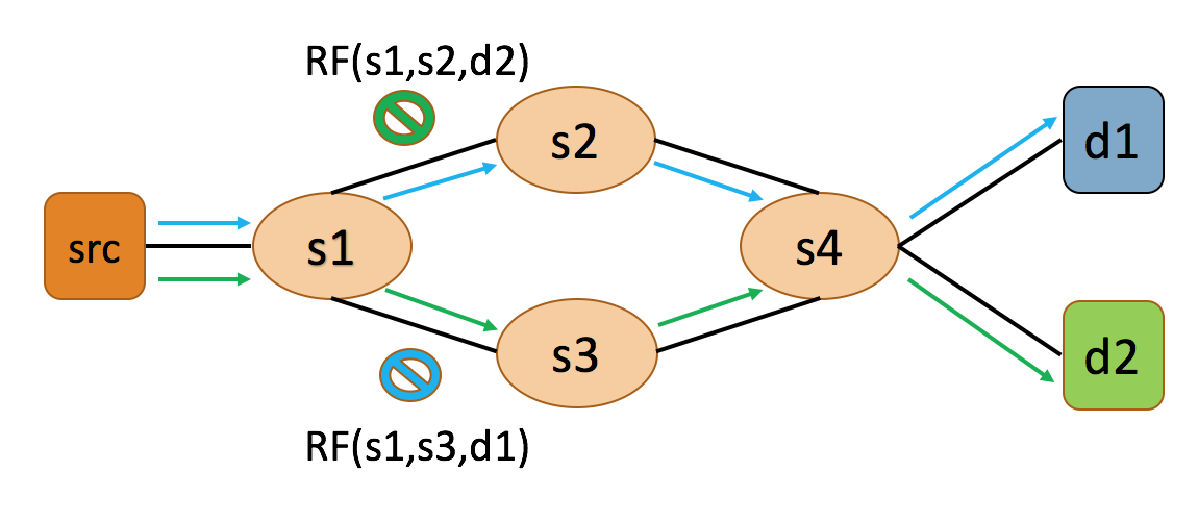
\includegraphics[width=\columnwidth]{figures/diamond.eps}
	\caption{Data plane example which requires route-filtering} \label{fig:diamond}
\end{figure}
Pure ARCs cannot be synthesized for all data planes. Consider the data
plane in \Cref{fig:diamond}. 
There exists no solution to the edge weights for this data plane. This is because 
there are two disjoint shortest paths connecting $s1$ and $s3$, and each path will have constraints
asserting it is the shortest of all paths. We define this structure as a \emph{diamond}. 
Formally,
consider two switches $s$ and $t$. There are two different destination DAGs with 
paths starting from $s$ such that they forward to different switches from $s$  
and these divergent paths from $s$ converge
at the switch $t$ first. 
\begin{theorem}
If the data plane contains a diamond, then no pure ARC  
can be synthesized for the data plane.
\end{theorem}
The converse is not true and discussed in <someplace>.

How does route-filtering work in this scenario? If we could disable the edge
$s1 \rightarrow s4$ for destination $s6$, then the ARC weights can be synthesized
such that $s1 \rightarrow s2 \rightarrow s3$ is taken, even if the actual shortest path
from $s1$ to $s3$ is via $s4$ and $s5$. Thus, by incorporating route-filters, we can
disable certain links in the topology for destinations, and increase the 
expressiveness of our synthesis. 
